\documentclass[../kl11.tex]{subfiles}
\graphicspath{{\subfix{../images/}}}

\begin{document}
\section{Substitution – radikal anders}

Wenn auch nicht immer auf den ersten Blick ersichtlich, findet man im Alltag mehr Radikalreaktionen, als man vermuten würde. So finden beispielsweise viele Oxidationsprozesse im menschlichen Körper über radikalische Prozesse statt. Aber auch die Industrie baut bei der Erzeugung einiger Werkstoffe auf Radikalreaktionen. Dennoch sind Radikale in der synthetischen organischen Chemie selten anzutreffende Vertreter. Jedoch kann man sich das außergewöhnliche Reaktionsverhalten auch in der organischen Chemie zu Nutze machen.

\enumaufgabe{\operator{Kreuze an}, ob die folgenden allgemeinen Aussagen über Radikale wahr oder falsch sind.
}
\renewcommand{\arraystretch}{1.2}
\begin{tabularx}{\textwidth}{|X|C{1.5cm}|C{1.5cm}|}\hline
    & wahr & falsch\\\hline
    Ein molekulares Radikal kann maximal ein ungepaartes Elektron enthalten. & \emptybox & \solutiontext{\checkedbox}{\emptybox} \\\hline
    Der Gesamtspin eines Radikals kann nur halbzahlige Werte annehmen. & \emptybox & \solutiontext{\checkedbox}{\emptybox}  \\\hline
    Radikale zeigen stets paramagnetische Eigenschaften. & \solutiontext{\checkedbox}{\emptybox} & \emptybox \\\hline
    Die Kunststoffe PE (Polyethylen) und PET (Polyethylentherephthalat) werden beide großtechnisch durch Radikalreaktionen hergestellt. & \emptybox & \solutiontext{\checkedbox}{\emptybox} \\\hline
\end{tabularx}
\solutiontext{je richtiges Kreuz 0,5 P. => 2P.
}{\vspace{0.5cm}}

Radikale gelten im Allgemeinen als sehr reaktive und daher sehr instabile Verbindungen. Dennoch gibt es einige Effekte, die die Stabilität von Radikalen begünstigen.
\enumaufgabe{\operator{Ordne} jeweils die folgenden Gruppen an Verbindungen vom instabilsten zum stabilsten Radikal.}

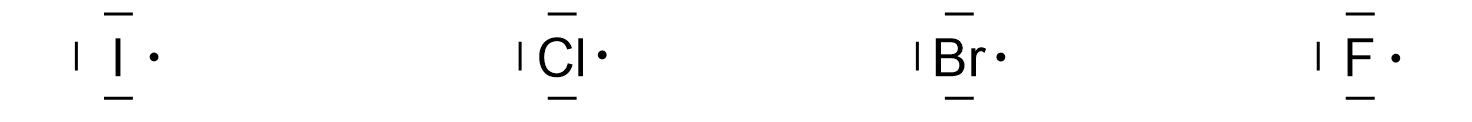
\includegraphics[width=\textwidth]{2024/Abbildungen/Radikal/1.jpg}\par
\begin{tabular}{L{0.035\textwidth}L{0.275\textwidth}L{0.245\textwidth}L{0.245\textwidth}L{0.068\textwidth}}
     I)&a&b&c&d  \\\hline
\end{tabular}

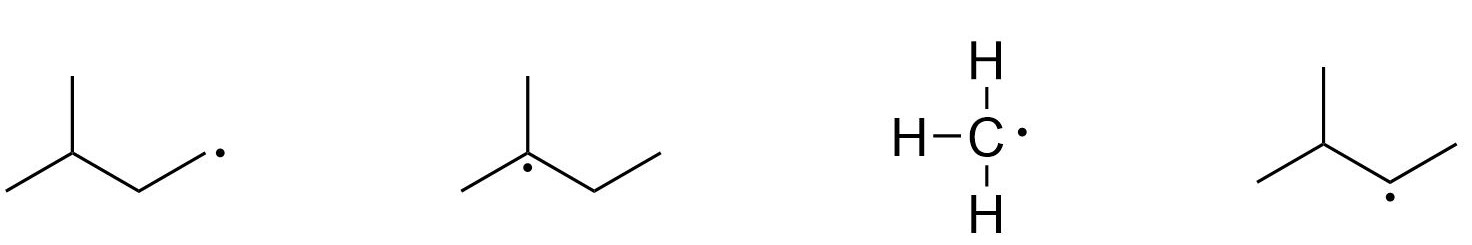
\includegraphics[width=\textwidth]{2024/Abbildungen/Radikal/2.jpg}\par
\begin{tabular}{L{0.035\textwidth}L{0.275\textwidth}L{0.245\textwidth}L{0.245\textwidth}L{0.068\textwidth}}
     II)&a&b&c&d \\\hline 
\end{tabular}

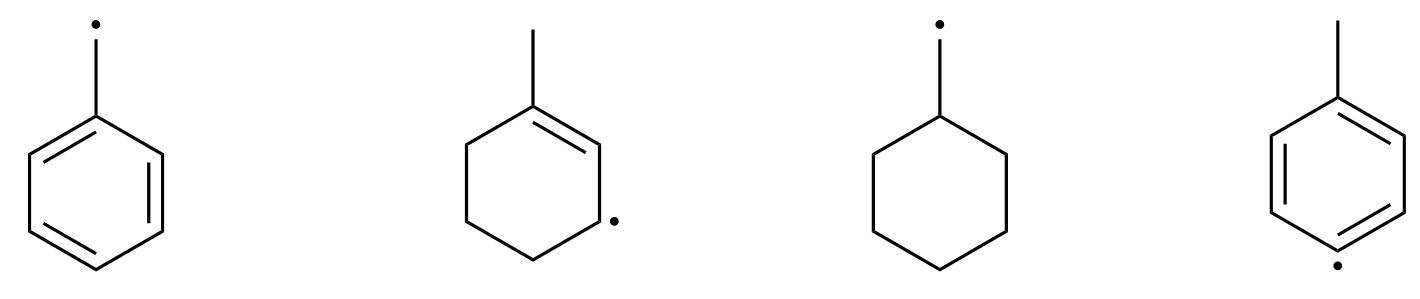
\includegraphics[width=\textwidth]{2024/Abbildungen/Radikal/3.jpg}\par
\begin{tabular}{L{0.035\textwidth}L{0.275\textwidth}L{0.245\textwidth}L{0.245\textwidth}L{0.068\textwidth}}
     III)&a&b&c&d  \\\hline
\end{tabular}
\newpage
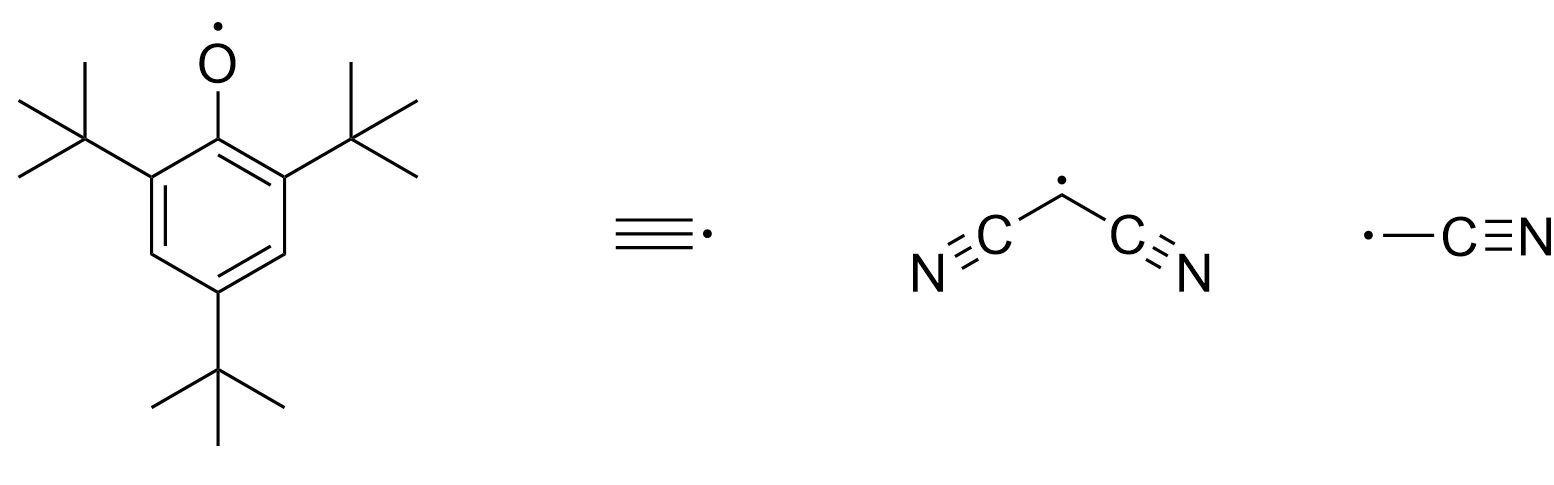
\includegraphics[width=\textwidth]{2024/Abbildungen/Radikal/4.jpg}\par
\begin{tabular}{L{0.035\textwidth}L{0.275\textwidth}L{0.245\textwidth}L{0.245\textwidth}L{0.068\textwidth}}
     IV)&a&b&c&d  \\\hline
\end{tabular}

\solution{
I) d, b, c, a \\
II) c, a, d, b \\
III) d, c, b, a \\
IV) b, d, c, a \\
Bewertung: Jedes richtig sortierte Paar gibt 0,25 P. Paare: a-b; a-c; a-d; b-c; b-d; c-d \\ 
insgesamt also 1,5 P. pro Gruppe \\
Besipiel: a, b, c, d ist richtig; Antwort ist c, b, a, d \\
Für a-b \& a-c \& b-c keine Punkte \\
Für a-d \& b-d \& c-d $3\cdot0,25=0,75$ P.\\
Insg. 6 P.}{4.5cm}



\textsc{Moses Gomberg} gilt als der Vater der Radikalchemie. Im Jahr 1900 synthetisierte und beschrieb er das sog. \textsc{Gomberg}-Radikal, welches als die erste Synthese eines Radikals betrachtet wird. Zwar wurde \textsc{Gomberg} für den Nobelpreis vorgeschlagen, verfehlte jedoch die nötige Anzahl an Stimmen knapp.
Das \textsc{Gomberg}-Radikal ist ein außergewöhnlich stabiles Radikal. Für die Synthese wird Tritylchlorid mit Silber umgesetzt. Es entsteht das \textsc{Gomberg}-Radikal und ein weißes Salz. Auch das \textsc{Gomberg}-Radikal kann dimerisieren, jedoch dimerisiert es nicht wie von Gomberg vermutet unter Rekombination der beiden ungepaarten Elektronen, sondern indem ein erstes Radikal das zweite Radikal in para-Stellung angreift. Das ungepaarte Elektron des zweiten Radikals bildet eine Doppelbindung im Dimer. Das Dimer hat genau einen $\mathrm{sp^3}$-hybridisierten Kohlenstoff.
\begin{figure}[H]
    \centering
    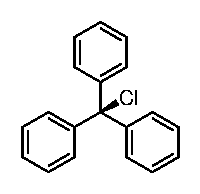
\includegraphics[width=0.3\textwidth]{2024/Abbildungen/Radikal/Tritylchlorid.eps}
    \caption{Tritylchlorid}
    \label{}
\end{figure}
\newpage
\enumaufgabe{\operator{Stelle} die Reaktionsgleichungen zur Synthese und zur Dimerisierung des Gomberg-Radikals unter der Verwendung der Strukturformeln der organischen Verbindungen \operator{auf}. \\Hinweis: Die Phenylgruppen können mit Ph abgekürzt werden.}

\solution{
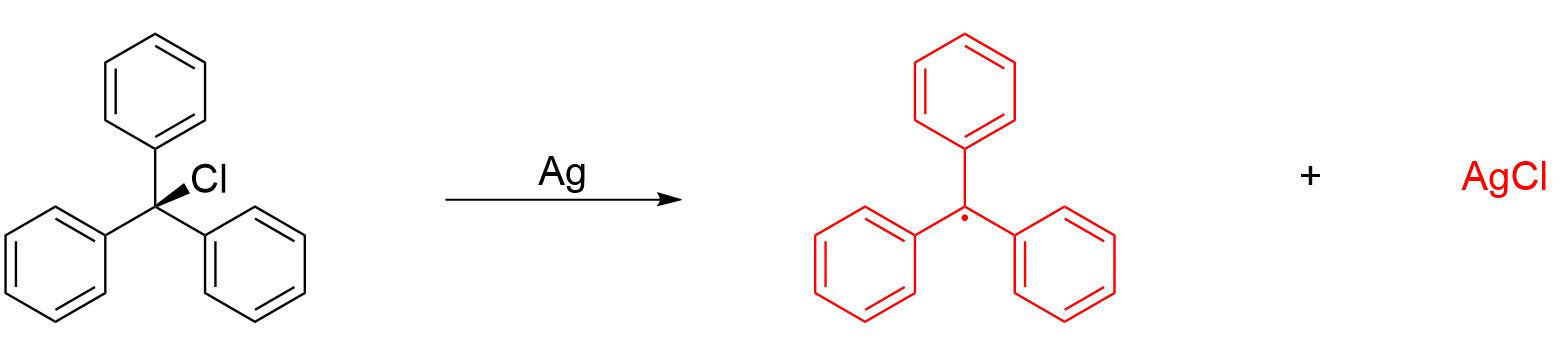
\includegraphics[width=\textwidth]{2024/Abbildungen/Radikal/Gomberg 1.JPG}
1 P. (Radikal) + 0,5 P. AgCl\\
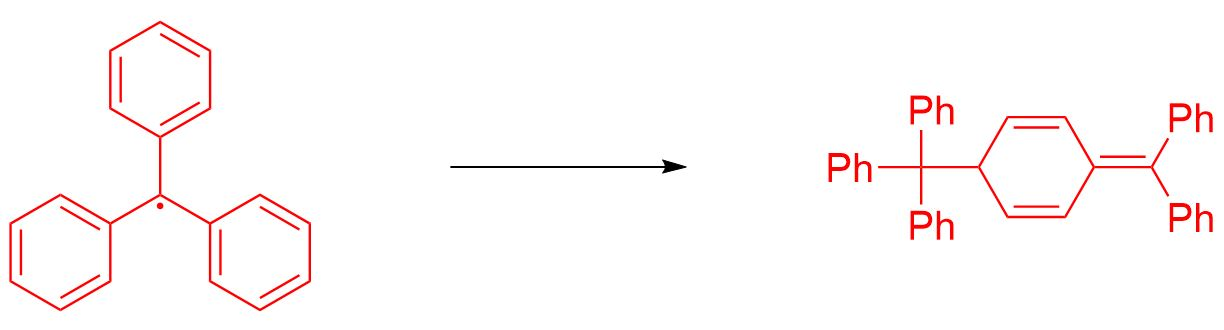
\includegraphics[width=0.82\textwidth]{2024/Abbildungen/Radikal/Gomberg 2.JPG} 1,5 P.\\
Insg. 3 P.}{9cm}

\enumaufgabe{\operator{Kreuze an}, ob die folgenden Aussagen wahr oder falsch sind.
}
\renewcommand{\arraystretch}{1.2}
\begin{tabularx}{\textwidth}{|X|C{1.5cm}|C{1.5cm}|}\hline
    & wahr & falsch\\\hline
    Das \textsc{Gomberg}-Radikal wird durch konjugierte Gruppen und sterische Abschirmung stabilisiert. & \solutiontext{\checkedbox}{\emptybox} & \emptybox \\\hline
    Das \textsc{Gomberg}-Radikal besitzt genau einen $\mathrm{sp^3}$-hybridisierten Kohlenstoff. & \emptybox & \solutiontext{\checkedbox}{\emptybox}  \\\hline
    Radikale werden durch elektronenziehende Substituenten stabilisiert. & \solutiontext{\checkedbox}{\emptybox} & \emptybox \\\hline
    Radikale werden durch elektronenschiebende Substituenten stabilisiert. & \solutiontext{\checkedbox}{\emptybox} & \emptybox \\\hline
\end{tabularx}
\solutiontext{je richtiges Kreuz 0,5 P. => 2P.
}{\vspace{0.5cm}}

Eine weitere interessante Eigenschaft von Radikalen besteht darin, Reaktionen mit Alkanen einzugehen. Über den Mechanismus der sogenannten radikalischen Substitution lassen sich so gesättigte Kohlenwasserstoffe funktionalisieren. Die Reaktionsfolge der radikalischen Substitution ist im Folgenden dargestellt:

\begin{figure}[H]
    \centering
    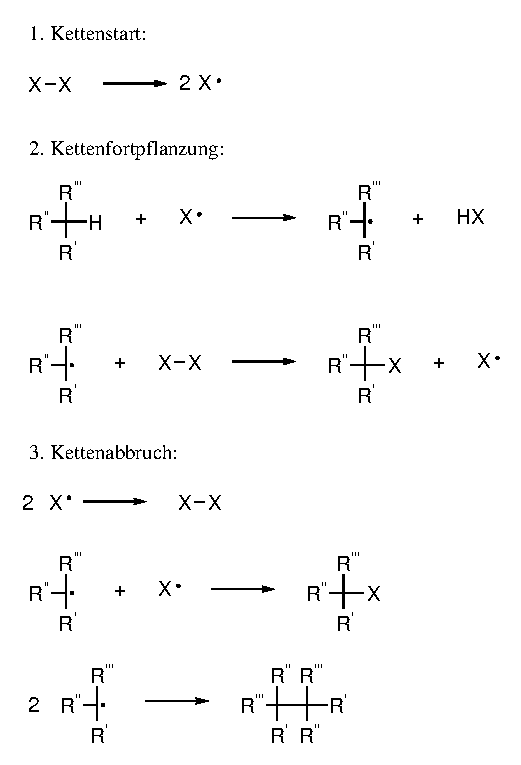
\includegraphics[width=0.5\textwidth]{2024/Abbildungen/Radikal/Reaktionsfolge radikalische Kettenreaktion[1].eps}
    \caption{Ablauf der radikalischen Substitution mit mit R‘-‚R‘‘-,R‘‘‘= Alkyl-/H-}
    \label{}
\end{figure}
Um eine radikalische Kettenreaktion in Gang zu setzen, braucht es im ersten Schritt zunächst einmal immer einen Radikalstarter. Bei einer radikalischen Halogenierung ist dies meist das Halogen selbst, bei welchem die Bindung photochemisch homolytisch gespalten wird. Ein anderer, sehr gängiger Radikalstarter ist AIBN, welcher bei seiner Zersetzung Stickstoff freisetzt.

\begin{figure}[H]
    \centering
    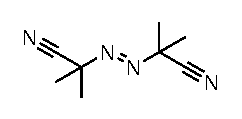
\includegraphics[width=0.4\textwidth]{2024/Abbildungen/Radikal/AIBN.eps}
    \caption{Struktur von AIBN}
    \label{}
\end{figure}
\newpage
\enumaufgabe{\operator{Stelle} unter Verwendung von Strukturformeln eine Reaktionsgleichung für die Zersetzung von AIBN \operator{auf}.}

\solution{\begin{figure}[H]
    \centering
    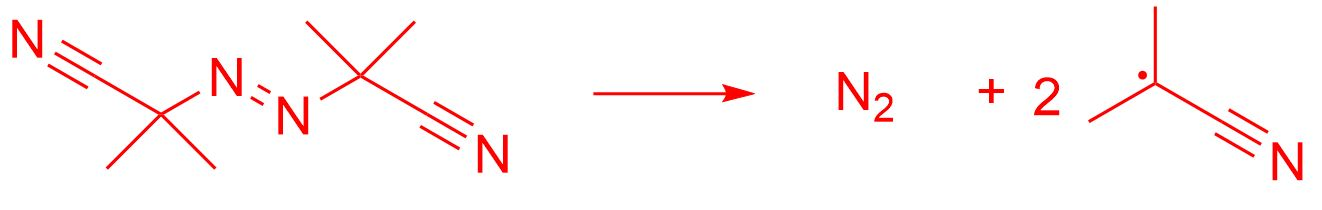
\includegraphics[width=\textwidth]{2024/Abbildungen/Radikal/AIBN.JPG}
\end{figure} 
1,5 P. auf Reaktionsgleichung
}{5cm}
\enumaufgabe{\operator{Begründe} stichpunktartig, warum es für die Zerfallsreaktion günstig ist, dass Stickstoff freigesetzt wird.}
\solution{- Freisetzung von Stickstoff begünstigt Zerfallsreaktion, da Gasfreisetzung entropisch günstig ist 
\\- Das Entweichen von \ce{N2} macht den Zerfall irreversibel\\
1 P. auf Begründung (eine reicht)}{3 cm}

Doch es ist nicht völlig zufällig, wo ein Radikal substituiert wird, es zeigt sich eine gewisse Regioselektivität. Das heißt, je nachdem ob es sich um ein primäres, sekundäres oder tertiäres Kohlenstoffatom im Molekül handelt, unterscheidet sich die Wahrscheinlichkeit, dass ein H-Atom an dem Molekül substituiert wird. 
\enumaufgabe{\operator{Gib} die Strukturformeln aller Isomere der Produkte \operator{an}, die bei der Monosubstitution von 1,1-Dimethylcy-clopentan mit Brom entstehen können. \\
\operator{Gib} für jedes Stereozentrum die absolute Konfiguration nach CIP \operator{an}.}

\solution{\begin{figure}[H]
    \centering
    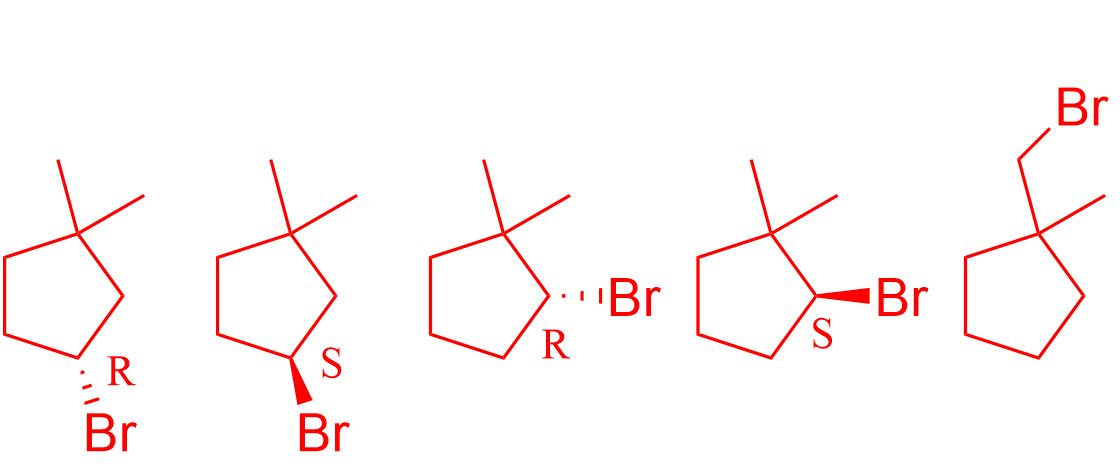
\includegraphics[width=\textwidth]{2024/Abbildungen/Radikal/Substitution.jpg}
\end{figure} 
0,5 P. für richtiges Edukt; 1 P. je Struktur und 0,5 P. je korrekter Konfiguration = 7,5 P. (bei falschem Edukt auch richtige Strukturen möglich)}{9 cm}

Für die Halogene konnten bei der radikalischen Substitution die folgenden relativen Reaktionsgeschwindigkeiten festgestellt werden:


\begin{tabularx}{\textwidth}{|X|X|X|X|}\hline
& primär &	sekundär &	tertiär \\\hline
Fluor & 1	& 1,2	& 1,4 \\\hline
Chlor	& 1	& 3,7	& 5 \\\hline
Brom	& 1	& 250	& 6300 \\\hline
\end{tabularx}
\ \\
Bei einer Reaktion von \SI{61,67}{\gram} 3-Ethylpentan mit Chlor hat man ein Stoffgemisch erhalten. Es konnte nachgewiesen werden, dass das Gemisch nur aus monochlorsubstituierten Produkten besteht. 

\enumaufgabe{\operator{Zeichne} die Strukturformeln aller Produkte des Gemisches.} 

\solution{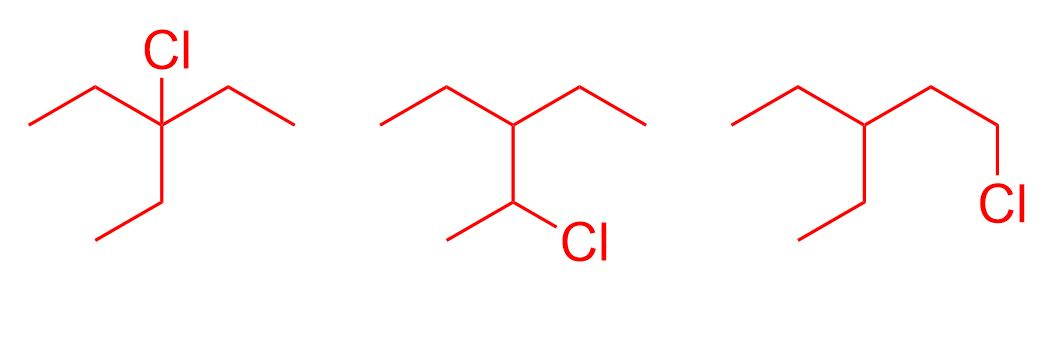
\includegraphics[width=0.9\textwidth]{2024/Abbildungen/Radikal/Produkte_Sub.jpg}\\
je Strukturformel 0,5 P. = 1,5 P.}{6 cm}

\enumaufgabe{\operator{Berechne} für jedes Produkt aus Teilaufgabe h) die Stoffmenge im Gemisch.}
\solution{
9 mal 1°:	 $9\cdot1=9$ \\
6 mal 2°:	$6\cdot3,7=22,2$ \\
1 mal 3°:	$1\cdot5=5$	 \\			
je Rechnung 0,5 P. \\
$$n_{1°}=\frac{9}{9+22,2+5}\cdot \frac{61,67 \thinspace\mathrm{g}}{100,205 \thinspace\mathrm{g/mol}}=0,153 \thinspace\mathrm{mol}$$ \\
$$n_{2°}=\frac{22,5}{9+22,2+5}\cdot \frac{61,67 \thinspace\mathrm{g}}{100,205\thinspace \mathrm{g/mol}}=0,3774 \thinspace\mathrm{mol}$$ \\
$$n_{3°}=\frac{5}{9+22,2+5}\cdot \frac{61,67 \thinspace\mathrm{g}}{100,205 \thinspace\mathrm{g/mol}}=0,085\thinspace \mathrm{mol}$$ \\
je 0,5 P. auf Ergebnisse, insgesamt 3 P.
}{8cm}



Auch der neuartige Stoff \textit{\textbf{Radikalium}} reagiert mit Alkanen unter einer radikalischen Substitution. Um die relativen Reaktionsgeschwindigkeiten $v_{\mathrm{rel}}$ an primären, sekundären und tertiären Kohlenstoffatomen bei der Umsetzung zu bestimmen, wird es mit 1,3-Dimethylcyclobutan zur Reaktion gebracht. Nach der Auftrennung und der Analyse des Reaktionsgemisches stellt man fest, dass \SI{50,04}{\milli\gram} des primär substituierten, \SI{166,8}{\milli\gram} des sekundär substituierten und \SI{150,12}{\gram} des tertiär substituierten Produktes entstanden ist. Die Analyse hat außerdem ergeben, dass nur monosubstituierte Produkte vorliegen.


\enumaufgabe{\operator{Berechne} die relativen Reaktionsgeschwindigkeiten $v_{\mathrm{rel}}$ für die radikalische Substitution mit \textbf{Radikalium} an sekundären und tertiären Kohlenstoffatomen. \\Hinweis: Beachte, dass die relative Reaktionsgeschwindigkeit an primären Kohlenstoffatomen auf eins normiert ist.}

\solution{
im Ausgansstoff: 6 mal 1°-, 4 mal 2°- und 2 mal 3°-H-Atome\\	
1 P. (nur wenn alles korrekt, sonst 0 P. und im Folgenden Folgefehler geben)\\
$$\frac{50,04}{6}=8,34$$    $$\frac{166,8}{4}=41,7$$      $$\frac{150,12}{2}=75,06$$ \\
1 P. (nur wenn alles korrekt, sonst 0 P. und im Folgenden Folgefehler geben)\\ \\
2°:     $\displaystyle\frac{41,7}{8,34}=5$  \\
3°:    $\displaystyle\frac{75,06}{8,34}=9$  \\
je 1 P. auf Ergebnis, insgesamt 4 P.
}{7.5cm}
\solutiontext{$\sum$ 31,5 P.}{}


\end{document}